%!TEX root = ../../thesis.tex
\define{\chapterpath}{\allchapterspath/introduction}
\define{\imgpath}{\chapterpath/img}

\chapter{Introduction}
\label{chapter:introduction}
\minitoc

% This thesis investigates how a robot can be taught what to do from instructions provided by a human without knowing beforehand how to associate the human communicative signals to their meanings.

In the past decades, robotics and autonomous systems have seen tremendous improvements in their motor, perceptual, and computational capabilities. As a good example, we have been able to send and operate rovers for several years on the planet Mars (Spirit, Opportunity, Curiosity), which indicates the technologies are well mastered. However, getting such robots to do what we want them to do remains a skill of few, and bringing robotics systems teachable by everyone and capable of social interaction in our daily life has been identified as the next milestone for the robotic community.

As for bringing computers in our homes required easy and intuitive ways for people to make use of them, bringing robots in our daily life requires easy and intuitive ways for people to instruct robots to do useful things for them. 
% Currently, implementing advance behaviors in a robot, such as folding a shirt, requires similar skills than a computer scientist needed 50 years ago to build an application using punch cards, i.e. a lot of expertise, patience and trials and errors development. 
But due to the diversity of skills a robot should be able to execute in our daily environment, including interacting with humans and objects, traditional programming methods hinder the deployment of robotic system at homes and workspaces.

Instead, researchers are trying to endow robotic systems with the ability to learn from social interaction.
% what tasks to execute and how they should be executed. 
Several methods have been considered to allow non-technical users to ``program'' robots, such as \emph{learning by demonstration} where a person demonstrates the skills to the robot, \emph{learning from reinforcement} where a person assesses the actions of the robot with respect to the aimed behavior, or \emph{learning from advice} where a person explains the sequence of actions to perform in order to fulfill a task.
% Advances in these areas should allow the emergence of robot companions, living inside our homes providing assistance to the daily tasks, care, and entertainment.

Endowing a robot with the ability to learn form interaction with a human requires to solve several challenges: the technical challenge of motor, perceptual, and cognitive skills acquisition and generalization, as well as the practical challenge of interacting in a social way with humans.
 % being of different background. 
Especially, the robot must be able to understand the communicative signals from the human.
% and communicate its own intention and ``state of mind'' back to the human. 

% Additionally, as robots are embodied agent, the social acceptance of robot among people is an additional obstacle. A robot that is not accepted by people will not be used, and a robot that cannot be understood by people or a non-intuitive interface is likely to impact the performances of the learning systems developed.

Currently most of these challenges are considered in isolation. For example, when a robot learns a task from human instructions, the robot receives instructions in a symbolic way, e.g. if the human uses speech to communicate his instructions, the robot is assumed to be able convert raw speech into text. Similarly, when a robot learns how to recognize speech utterances, which is how to convert raw speech into a meaningful representation, such as text, the robot is usually fed with many examples of speech utterances associated with their symbolic representation.

In this thesis, we consider the two latter challenges simultaneously, which is learning a new task from raw human instruction signals whose associated meanings are initially unknown. Solving this problem would allow the same robot to be taught by a variety of users using their preferred teaching signals, and without the intervention of an expert to calibrate the system 
% to the specific teaching signals of 
for each users. For example, a robot that accepts speech commands usually accept only one or a limited set of pre-specified speech utterances for each command, e.g. using the word ``forward'' to ask the robot to move forward. With the method described in this thesis, the user could use its preferred word to ask the robot to move forward, e.g. ``straight'' or ``up'', but also words whose usual meanings are non-related to the move forward action such as ``dog'', ``backwards'', or ``blue'', or interjection such as ``ah'', ``oh'', or even non speech utterances such as a hand clapping. The robot, after some practical interaction with the user, will find out which signal is associated to the action moving forward.

% Our approach assumes the robot has access to a limited set of task hypotheses, which include the task the user wants to solve. For example, if the user's goal is to guide the robot towards a specific room in a house, there are a limited number of possible tasks, which are the number of rooms in the house. The idea behind our method consists of generating interpretation hypotheses of the teaching signals with respect to each hypothetic task. We will see that by building a set of hypothetic interpretation, i.e. a set of signal-label pairs for each task, the task the user wants to solve stands out by having the best coherence between the underlying spacial organization of the signals in their feature space and the labels associated to each signal. In others words, the correct task is the one that explains better the history of interaction.

In the following of this introduction, we present in more details the challenges of learning from social interaction with humans and explicit the usual assumptions made when designing such systems. On this basis, we define the specific challenge of \emph{learning from unlabeled interaction frames} 
% addressed in this work 
and present the contribution of the thesis.

%%%%%%%%%%%%%%%%%%%%%%%%%%%%%%%%%%%%%%%%%%%%%%
%%%%%%%%%%%%%%%%%%%%%%%%%%%%%%%%%%%%%%%%%%%%%%
%%%%%%%%%%%%%%%%%%%%%%%%%%%%%%%%%%%%%%%%%%%%%%
%%%%%%%%%%%%%%%%%%%%%%%%%%%%%%%%%%%%%%%%%%%%%%
%%%%%%%%%%%%%%%%%%%%%%%%%%%%%%%%%%%%%%%%%%%%%%
\section{Social Learning: Robot learning from interaction with humans}
\label{sec:intro:social}

It is often easier to acquire a new skill if someone that has already acquired that skill teaches us how to do it. The field of social learning in robotics investigates how knowledge can be transferred from humans to robots through social interaction. Social interaction implies that the human interacts with the machine using similar modalities as when interacting with other human beings, for example using speech, gestures, or by demonstrating some behaviors.

We can identify three main social learning paradigms used in robotics today: \begin{inparaenum}[(a)] \item learning from human demonstration, where the robot learns by imitating the human actions, \item learning from human reinforcement, where the robot learn from assessments on its own actions provided by the user, and \item learning from human advice, where the robot learns from concrete instructions about what do to next provided by the user. \end{inparaenum}

Each of these paradigms requires to solve two main challenges: \begin{inparaenum}[(1)] \item the robot must be able to identify which parts of the interaction, and of the environment, are relevant to the acquisition of the new skill, and \item the robot must be able to infer, from the relevant information extracted from the interaction, the new skill, or task, the human wants the robot to achieve. \end{inparaenum}

As we will see in the following subsections, most of the work in robot social learning considered these two latter challenges separately and most of the efforts focused on the second challenge of learning a new skill from pre-formatted data.

% This approach contrast with the usual methods used to endow a robot with a new skill, such as directly programming the robot or defining a mathematical fitness function for that skill. 
% Social interaction, by being the most intuitive way for humans to communicate, are the most intuitive way human communicative between each others and if robot are able
% By using speech, gestures, or by providing demonstration, human users can teach a robot a new skill without knowing how to program or how to define a fitness function this a particular skill. 
% This way human users can interact with machines without knowing how to program or how to define a fitness function for a particular task. People will be more familiar of the desired skill, which correspond to more intuitive interaction for humans.

% In the following of this section we present three main social learning paradigms: \begin{inparaenum}[(a)] \item learning from human demonstration, where the robot learns by imitating the human actions, \item learning from human reinforcement, where the robot learn from assessments on its own actions provided by the user, and \item learning from human instructions, where the robot learns from concrete instructions about what do to next provided by the user. \end{inparaenum}

%%%%%%%%%%%%%%%%%%%%%%%%%%%%%%%%%%%%%%%%%%%%%%
%%%%%%%%%%%%%%%%%%%%%%%%%%%%%%%%%%%%%%%%%%%%%%
\subsection{Learning from human demonstrations}

Learning from human demonstrations, also called programming by demonstration or learning by imitation, is the process of learning a new skill from practical examples of how to perform that skill \cite{schaal1999imitation,calinon2008robot,argall09survey,lopes10imitationchapter}. More formally, the robot must infer a policy that is a mapping between world states and actions by observing only some, potentially noisy, examples of state to action mapping. %, i.e. some demonstrations, which may be noisy and incomplete.

Following the survey of Argall \cite{argall09survey}, we segment our presentation of learning from human demonstration in three parts, first we present the different methods used to collect training data, i.e. to gather the demonstrations, then we present several methods allowing to derive a policy from demonstration, and finally we highlight some limitations of the method.

% Demonstrating a task to a robot is easier for the user than directly programming a behavior by writing lines of code. But creating a robot that learn from example requires to solves two main problems: \begin{inparaenum}[(1)] \item creating algorithm capable of inferring the user desired behavior from its demonstrations, but also \item allowing the robot to identify what part of the environment and of the human behavior are relevant to the task, i.e. to extract the information related to a demonstration from the interaction. \end{inparaenum}

\subsubsection*{Collecting demonstrations}

Collecting demonstrations is probably the most important part in the learning process. Demonstrations of good quality will result in an easier learning while bad quality demonstrations are likely to impact the quality of the learned behavior.

We group the demonstration recording methods in two categories: \begin{inparaenum}[(1)] \item by teleoperation, where the human demonstrate a skill by directly controlling the robot, and \item by external observation, where the robot is observing the human providing demonstration. \end{inparaenum} More formally, learning from data collected by a direct control of the robot by the human is called learning from demonstration, while learning from data collected by observing the human demonstrating the skill is called learning from imitation. 
% We will see that this latter approach raises some embodiment issues.

During teleoperation, the robot is directly operated by the teacher and therefore records the demonstration using its own sensors, i.e. the robot directly observes a sequence of state-action pairs in its own referential. It is the most direct and most precise method to provide demonstrations. However this method does not always apply well to robots. For example, robots with many degrees of freedom cannot be teleoperated efficiently by one person, but also robots that should maintain equilibrium are sometimes impossible to manipulate directly, such as demonstrating a walking behavior by teleoperating the legs of a humanoid robot.

Teleoperation has been used in a variety of robotic applications, including learning of aerobatic helicopter flight \cite{abbeel2007application}, object displacement with environmental constrained (e.g. obstacle avoidance) \cite{guenter2007reinforcement,calinon2007teacher}, object stacking \cite{calinon2007teacher}, or ball grasping on the Aibo robot \cite{grollman2007learning}.

When learning by imitation, the robot observes a human teacher demonstrating the skill. The fundamental difference with the teleoperation approach is the difference of embodiment between the human and the robot. This issue is referred as the correspondence problem \cite{nehaniv2002correspondence}, which is the problem of mapping between the demonstrator actions (i.e. the human) and the imitator actions (i.e. the robot). For example, when demonstrating a gesture to a humanoid robot, as the human and the robot do not share the same body characteristics, the robot cannot directly transpose the human movement to its own body. If we consider a humanoid robot imitating the posture of a human demonstrator, the problem is better defined as reproducing the human posture as closely as possible while maintaining balance \cite{hyon2007full,yamane2009simultaneous}, where the system designer provides some additional constraints to the robot.

Recording the human demonstration can be done using a variety of sensors, either by adding sensors directly on the users (wearable sensors), either by using only sensors remotely observing the demonstrator body or relevant objects, for example using a motion capture device or using a pair of video cameras.
 % situated in the robot's head.

Learning by imitation has been investigated in a variety of robotic applications, including executing a tennis forehand swing \cite{ijspeert2002movement}, imitating arm movement \cite{billard2001learning} and hand posture \cite{chella2004posture}, object grasping \cite{lopes2005visual,tegin2009demonstration}, but also demonstration including a force component such as the fingertip force for grasping and manipulating objects \cite{lin2012learning}. Other works focused on learning by imitation a sequential task, which required combining a sequence of multiple actions to fulfill the task \cite{pardowitz2005learning,natarajan2011imitation}.

\subsubsection*{Inferring a policy}

Given a dataset of demonstrations collected using one of the methods presented above, the robot should infer what action it should take in any given state to correctly fulfill the task demonstrated by the human. This process can be as straightforward as reproducing the demonstrated behavior exactly. But most often, as the demonstrations may be noisy or incomplete, the robot needs to learn and generalize from these examples. We will differentiate between two approaches: \begin{inparaenum}[(a)] \item directly deriving a mapping between states and actions, i.e. a policy, from the observed data with the aim or reproducing the teacher policy, and \item inferring the human objective and reproducing the desired outcome without necessarily using the same actions as the demonstrator. \end{inparaenum} Roughly, the first approach is more suited for imitation, which is the act of reproducing the human demonstration in all details, while the second is more suited for emulation, which is the act of fulfilling the same goal as the human.

The first approach resumes in approximating the policy function observed form the user behavior. Depending on the properties of the problem, the algorithms for learning the policy are either classification or regression techniques. 

\begin{itemize}

\item \textbf{Classification} methods are well suited for mapping discrete or continuous states to discrete actions. An example would be a robot learning to play a video game from demonstration in which, depending on the current state of the agent in the world, the robot should learn to press the appropriate buttons.

A large variety of classification algorithm has been used in learning form demonstration scenario. Among others, Support Vector Machines were used for a robot learning how to sort balls \cite{chernova2008teaching}, Hidden Markov Models have been used for an assembly task \cite{hovland1996skill}, Gaussian Mixture Models in a simulated driving domain \cite{chernova09jair}, but also neural networks \cite{mataric2000sensory}, beta regression \cite{montesano2009learning} or k-Nearest Neighbors \cite{saunders2006teaching}.

\item \textbf{Regression} method are well suited for mapping discrete or continuous states to continuous actions. An example would be an autonomous car learning to steer the wheels from demonstration, given information about the surrounding environment the car should turn the driving wheel appropriately.

A large variety of regression algorithm has been used in learning form demonstration scenarios, they were mainly applied for learning trajectories from noisy demonstrations. Among others, Gaussian Mixture Regression for generalizing trajectories from examples in different applications \cite{calinon07}, Locally Weighted Regression for learning to produce rhythmic movement using central pattern generators \cite{schaal1998programmable,ijspeert2002learning}, Neural Networks for learning autonomous driving \cite{pomerleau1991efficient}, or Incremental Local Online Gaussian Mixture Regression for imitation learning for learning incrementally and online new motor tasks from demonstration \cite{cederborg2010incremental}.

\end{itemize}

The second approach consists of inferring the goal of the human from demonstration. By expressing this goal as an optimization problem or as a reward function, the robot can learn to reproduce the human goal by its own means.

Inverse reinforcement learning \cite{ng2000algorithms,Abbeel04icml,macl09airl} is a popular method that is inferring the hidden reward function the demonstrator is trying to optimize based on the observation of its actions. In addition, the human demonstrations can be used to learn a model of the environment in state unreachable to robot by mere self-exploration. Once the reward function has been evaluated form the demonstrations, and given the dynamic of the environment, the robot can generate a plan to fulfill the task using its own ability. This method is especially interesting when the human and the robot do not have the same abilities. As an example, a robot may be able to execute a skill faster that a human, but by mere reproduction of the human gestures the robot would not reach the same level of performance than by inferring the underlying goal of the human and solving the problem its own way.

One of the most impressive achievement of the past decade used inverse reinforcement learning methods for the learning of aerobatic helicopter flight \cite{abbeel2007application}. Demonstration were provided by an expert pilot teleoperating, i.e. flying, the helicopter to help finding its dynamics and the fitness function corresponding to different maneuvers such as flip, roll, tail-in and nose-in funnel.


\paragraph{} Finally, in the work of Lopes et al. \cite{lopes2009computational}, the authors propose to combine imitation and emulation in a unified model by considering a continuum space whose three extreme cases are non-social behavior, emulation, and imitation. A demonstration from a teacher is evaluated according to these three baseline, and the agent final policy is a combination, more precisely a weighted mixture, of the three modules. By varying the weight attributed to each module, they were able to reproduce several well-known social learning experimental paradigms.

% proposing a computational model to \textit{``describe how observed behavior can influence an observer’s own behavior, including the acquisition of new task descriptions''}. They propose a unified model for social learning as 

\subsubsection*{Limitations and assumptions}

The performance of a learning system is obviously linked with the quality of the information provided by the demonstrations. Among others aspects, if some important state-action pairs have not been demonstrated or if the demonstrations were of poor quality, i.e. including a lot of noise or being suboptimal or ambiguous in certain areas, the learner will be unable to generalize properly from the data. 

Unfortunately, in many cases, the demonstration are collected beforehand and sent to the learning algorithm in a batch way which do not allow the robot to have access to better demonstration. A potential solution is to ask the teacher for new demonstrations in those state where demonstration are missing or uncertain \cite{chernova2008multi,chernova09jair}, we will detail more this approaches in the next chapter.

Another problem is that of identifying what the human is really demonstrating. For example, if a human is demonstrating how to fish to a robot, is the human demonstrating the precise movement of the fishing rod or is he demonstrating where to place the float in order to catch more fish. In other words, should the robot imitate the movement of the fishing rod or should it emulate the position of the float. Where imitation is the act of reproducing the human demonstration in all details, and emulation is the act of fulfilling the same goal as the human.

This problem is currently unsolved in the robot social learning literature and in practice the robot is explicitly told whether to imitate or emulate the demonstration. The problem of understanding what to do from the interaction with human is usually solved at design time; where the system designer applies a multitude of constraints to the interaction with the robot such that no uncertainty or ambiguity remains on the demonstrations. For example, the demonstrated movements are provided in isolation and contain only information about the task to be learned. Similarly, the robot is explicitly ``told'' that the demonstrations refer to such and such objects and that it is for example a grasping task. Of course saying that the robot is ``told'' about the interaction is misleading; it is rather the all system that is constrained to optimize only a specific objective.

In the context of learning from human demonstration, four central questions are often predefined at design time: who, when, what, and how to imitate \cite{nehaniv2000hummingbirds}:

The \textbf{who} question refers to the problem of identifying who to imitate. It may refer to finding that a person is currently providing demonstrations, but also which person is better at providing accurate demonstrations of the task. This question has not been thoroughly investigated in the literature so far. One of the few work tackling this problem consider a finite set of teacher and select the most appropriate one based on the robot current learning rate \cite{Nguyen2012PJBR}. This method allows the robot learner to take advantage of the different levels of skills each teacher provide.

The \textbf{when} question refers to the problems of social coordination between the two partners, such as the turn-taking ability. For example, this aspect has been investigated in human-robot drumming activities where turn taking and role switching are important component of a successful interaction \cite{weinberg2006robot,kose2008emergent}. The when question also applies for cases where the robot should decide whether to try to imitate its human partner or to explore the environment by itself \cite{chernova09jair,Nguyen2012PJBR}. 

The \textbf{what} question refers to the problem of identifying the important aspect of the demonstrations. It refers for example to the dilemma between imitation at the action level and emulation at the effect level. At the action level, the aim of the robot would be to reproduce the demonstrator action in the same way and in the same order. At the effect level, the robot should understand the underlying purpose associated to the actions of the human.

The latter problem of identifying the effect level of imitation depends on the context in which the interaction takes place. In particular the concept of affordances \cite{gibson1986ecological} --- which encode the relation between actions, objects and, effects --- is of primordial importance for the robot to be able to reproduce demonstrations at the effect level. Several works have consider affordances for human-robot learning, among others they have been used to recognize demonstrations, decompose them in a sequence of subgoals and finally reproduce them \cite{macl07affimit}. Montesano et al. presented a method to learn affordances by interacting with several objects \cite{montesano2008learning}. The robot was able to extract relation between its actions, the objects, and the effects they produces using Bayesian inference methods.

While most of the time the interaction protocol is well constrained such that there is no ambiguity about what aspects of the demonstrations should be imitated, some social cues can be used to infer which parts of a demonstration are relevant, such as the temporal differences of demonstration parts. Pauses during interaction have been linked to important key points in a task demonstration. This allows for example to extract subgoals or determine when a demonstration is completed \cite{theofilis2013temporal}.

The \textbf{how} question refers to the problem of determining how the robot will actually perform the behavior so as to conform with the metric identified when answering the what question. When the demonstration is only relevant at the effect level (emulation) the robot can solve the task by its own mean as soon as the objective is identified. However when the imitation is important at the action level (imitation), differences between robot and human morphology and capabilities makes solving the how question not straightforward. This latter issue has been discussed previously and is referred to as the correspondence problem \cite{nehaniv2002correspondence}, which the problem of mapping between the demonstrator and the imitator.

\transition

As stated before, the who, when, what, and how questions are usually skipped over in practical application and the data are provided already pre-formatted for the robot.

In the next subsection we present another paradigm for social learning in robotics, the \emph{learning from human reinforcement} approach. In this paradigm, the human never demonstrates the task to the robot but rather observe the behavior of the robot and reinforces or punishes some of its actions in order to shape its final behavior. We also call this approach learning from human feedback, where feedback implies a positive or a negative assessment of the robot's actions.

%%%%%%%%%%%%%%%%%%%%%%%%%%%%%%%%%%%%%%%%%%%%%%
%%%%%%%%%%%%%%%%%%%%%%%%%%%%%%%%%%%%%%%%%%%%%%
\subsection{Learning from human reinforcement}

Learning from human reinforcement, also called shaping, is the process of learning a new skill by receiving assessment over recently performed actions. In this paradigm, the human never demonstrates the task to the robot but he rather observes the behavior of the robot and reinforces or punishes some of the robot's actions in order to shape its final behavior. We also call this approach learning from human feedback, where feedback implies a positive or a negative assessment of the robot's actions. Clicker training \cite{kaplan2002robotic} is a subclass of this problem that considers the human can only send positive reinforcement.

Pioneer works in this domain include the work of Blumberg et al. \cite{blumberg2002integrated} that trained a virtual dog to learn several sequential tasks and associate them with verbal cues using clicker training method. Kaplan et al. \cite{kaplan2002robotic} applied similar methods to train an AIBO robot dog. Another pioneers work considered a software agent, named Cobot, which interacts with human agents in an online chat community called LambdaMOO. Cobot adapts its behavior from various sources of feedback (reward or punishment) provided by human engaged in the chat community \cite{isbell2001social}.

This social learning paradigm shares many aspects with reinforcement learning \cite{sutton1998reinforcement}. In reinforcement the agent goal is to take actions so as to maximize the cumulative reward. We make a difference between reinforcement learning algorithm and learning from human reinforcement in the sense that the nature of the reward information cannot be treated the same way when a human provides it. For example, reward signals from humans are frequently ambiguous and deviates from the strict mathematical interpretation of a reward used in reinforcement learning \cite{thomaz2008teachable,Cakmak2010optimality}. We will provide more detail about the teaching behaviors of humans in the next chapter but we note that this problem requires developing new algorithms to monitor and handle the teaching style of each user.

Therefore recent works started to investigate how to additionally learn the way humans provide feedback at the same time as the robot learns the skill \cite{knox2009interactively}. 

However, as for learning from human demonstration, the robot should be able to answer the who, when, what, and how questions. It needs to infer to which actions the human feedback relates to, but it also needs to differentiate between different levels of feedback as some actions may be mandatory to complete the task while others may just be preferences from the users. In addition the user could make mistakes in its assessment or may not perceive the problem as the robot perceives it, therefore making inconsistent feedback. And as for most learning from demonstration systems, most of the works presented above consider predefined and restricted interaction protocols so as to be able to map easily the human reinforcement with the robot's actions. Similarly, if the human is providing feedback using speech commands, there exist system translating speech utterances into meaningful feedback, e.g. mapping the word ``good'' to a positive reward.

\transition

As stated above, the who, when, what, and how questions are also applicable to learning from human reinforcement. This question is usually skipped over in practical applications by providing already pre-formatted data to the robot.

Providing only reinforcement signals to a robot can be limiting, especially when the state space is large increasing the learning time and resulting in a laboring interaction between the human and the robot. In the next subsection we present another paradigm for social learning in robotics, the \emph{learning from human advice} approach. In this paradigm, the human never demonstrates the task to the robot but rather observes the behavior of the robot and provides hints about what action to perform next, which we will call guidance.

%%%%%%%%%%%%%%%%%%%%%%%%%%%%%%%%%%%%%%%%%%%%%%
%%%%%%%%%%%%%%%%%%%%%%%%%%%%%%%%%%%%%%%%%%%%%%
\subsection{Learning from human advice}

Learning from human advice, also called learning from instruction, is the process of learning a new skill by receiving explicit instructions about what to do next. In this paradigm, the human never demonstrates the task to the robot. It rather observes the behavior of the robot and provides clues accordingly in order to shape the robot final behavior. We also call this approach learning from human guidance, where guidance implies that the user explicitly indicates to the robot what action to perform next.

In most scenarios, advices are additional pieces of information improving the learning time and efficiency of an agent. It is therefore often combined with reinforcement learning algorithms where the advices influence the exploration behavior of the agent or influence directly the value of particular actions. 

In \cite{clouse1992teaching} and \cite{maclin2005giving} the teacher can influence the action selection of the agent by providing advices about preferred actions. In  \cite{smart2002effective} the trainer directly controls the agent's actions at important key states and let the agent learns the fine details. In \cite{kolter2007hierarchical}, the authors introduce a hierarchical apprenticeship learning method for teaching a quadruped LittleDog robot to walk on rough terrains. Their method differs from standard inverse reinforcement learning methods. Rather than providing full demonstrations of the skill, they use human advices about low-level actions of the problem. More precisely, the human expert indicates foot placement in situation where the robot made suboptimal footsteps.

It is important for the robot to be able to generalize to unseen situations. In \cite{lockerd2004tutelage}, the robot Leo learns to switch all buttons on or off from human vocal instructions. When a new button is introduced in the environment the robot autonomously generalizes from the instructions and presses all buttons, instead of pressing only the ones it was instructed to in the first place.


As for other learning paradigms, the robot should be able to answer the who, when, what, and how questions. It should infer which part of the environment matters for the advices, if the advices can be generalized or not to other objects in the environment, if the advices are related to what the robot should do next or what it should have done before, or in which referential are the advices given. Ideally the robot should also keep track of other social signals from the human, such as whether the user is really paying attention to the scene.  Or whether the user can see the part of the space the robot is in. Most of the time predefining and restricting the interaction protocols solve these problems.

\subsection{Discussion}

Our categorization of social learning paradigms in three categories does not reflect the many subfamilies that exist inside these categories, including those that are shared among categories. It is meant to situate the social learning problem in a more global picture, providing some interesting pointers for the interested readers. 

As we noticed, in most of the above presented work, the human had either no direct interaction with the robot, either few highly constrained interactions. For example, the human demonstrations are provided in a batch perspective where data acquisition is done before the learning phase. In the following section, we detail the usual assumptions made in most human robot interaction scenarios.  Based on our observations we then define the global challenges addressed in this thesis.

%%%%%%%%%%%%%%%%%%%%%%%%%%%%%%%%%%%%%%%%%%%%%%
%%%%%%%%%%%%%%%%%%%%%%%%%%%%%%%%%%%%%%%%%%%%%%
%%%%%%%%%%%%%%%%%%%%%%%%%%%%%%%%%%%%%%%%%%%%%%
%%%%%%%%%%%%%%%%%%%%%%%%%%%%%%%%%%%%%%%%%%%%%%
%%%%%%%%%%%%%%%%%%%%%%%%%%%%%%%%%%%%%%%%%%%%%%
\section{Usual Assumptions}

% In this thesis we focus on the learning from human reinforcement paradigm, which we will refer to as learning from feedback signals, and the learning from human advices paradigm, which we will refer to as learning from guidance signals. For convenience we will refer to both feedback and guidance signals as instructions signals, in the sense that a teacher is instructing the robot using signals that may includes both feedback or a guidance instructions towards a final goal.

As seen in the previous section, there is usually a strong decoupling between the process of extracting useful information from the interaction and the process of learning a new skill from those information. We can already highlight a chicken and egg problem in the social learning literature:

\begin{itemize}

\item On the one hand, if the goal of the robot is to learn a new task, the robot will be fed with the relevant data formatted exactly as needed by the learning algorithm. For example, if a user teaches a robot to navigate in a maze, the protocol of interaction will be fixed to match the need of the algorithm. The interaction will be done turn by turn such as it is easy to associate user's instructions to robot's states. But the user will also be asked to comply to the specific signals the robot understands, such as using the word ``right'' and ``left'' to mean respectively ``right'' and ``left''.

\item On the other hand, when we want to learn the user behavior or the protocol, we assume the task the users wants to achieved is known. It allows interpreting the behavior of the user in light with the known objective he is pursuing. This process is usually called a calibration phase. It is for example necessary to provide the robot with the ability to translate human communicative signals, such as speech or gestures, in a symbolic meaningful representation. For example, if we want our robot to learn which words the human uses to mean ``right'' and ``left'', we will ask the user to guide the robot in a maze following a specific path. The robot, knowing the path intended by the human, could identify that the human uses the word ``right'' and ``left'' or ``droite'' and ``gauche'' to mean respectively ``right'' and ``left''.

\end{itemize}

To summarize, in order to teach a robot a new task, the robot must be able to understand the behavior of the human. But to come up with an understanding of the behavior of the human, the robot must know what is the user overall objective. In this thesis, we present methods to overcome this chicken and egg problem in some specific cases. This allows a user to start interacting with a machine using its own preferred signals; removing the need for a calibration procedure. Before entering into more detail, we introduce the concept of interaction frames.

\subsection{Interaction frames}

An interaction frame \cite{rovatsos2001interaction} is a structure that defines all the aspects of the interaction that are pre-defined by the system designer. This interaction schema is assumed to be followed by the human and known by the robot.

The concept of interaction frame is a subclass of the more general concept of frame. Frames are a concept that emerges simultaneously in social theory \cite{goffman1974frame} and artificial intelligence \cite{minsky1974framework}. They represent a schema of interpretation given a particular situation or event. It is answering the question: \emph{what is going on here ?}, in order to reduce ambiguity of intangible topics by contextualizing the information. It creates a common ground about the purpose of the interaction \cite{tomasello2009cultural,rohlfing2013learning} and includes ``predictable, recurrent interactive structures'' (\cite{ninio1996pragmatic}, p. 171). 

In \cite{rovatsos2001interaction}, Rovatsos et al. presented an extended definition of what an interaction frame might be for artificial agents. While his definition can be transposed to human-robot interaction scenarios, its description and formalization of interaction frames is too much detailed for our forthcoming development. To summarize, an interaction frame provides interactants with guidelines about how to behave (a protocol for interaction). It also allows interactants to understand the communicative intentions of their interaction partner. The interaction frame is often implicitly defined and known in robot learning experiments. We exemplify a few interaction frames and then provide our simplified description of an interaction frame.

\paragraph{Naming frame} One example of an interaction frame are found in language games \cite{steels2002aibos}, where a pre-defined sequence of interaction is defined to associate a name to an object. For example, a human presents an object to a robot and pronounce the name of that object. Being aware of this frame, the robot knows that speech of the human corresponds to the name of the object (and not its shape or its color). In addition the interaction is usually well controlled. The human will first hand the object in front of the robot. The robot will then ask always the same question such as \emph{``tell me the name of this object?''}. Once the robot is ready to accept the human speech utterance, it emits a small noise.  Finally the human speaks for one second. Following this sequence, the association between objects and names is guaranteed to be unambiguous.

\paragraph{Feedback frame} 

To exemplify the feedback frame, we introduce the navigation task used for our brain computer interaction experiments chapter~\ref{chapter:lfui}. In this scenario a human assesses the actions of a virtual agent in a gird world (see Figure ~\ref{fig:feedbackBCIexample}). The human wants to guide the agent towards a specific state. To do so he can send to the agent information about the correctness of its last action. For example, if the robot went away from the target state, the human informs the robot that going North was ``incorrect'' according the target. After several interactions the robot is able to identify the goal state. We call this specific interaction scenario a feedback frame. A feedback signal is providing information about the optimality of the robot's last action. A feedback signal can only take two values, ``correct'' or ``incorrect''. In practice the interaction is turn taking, the robot performs one action and waits until the human provides a feedback signal. That way the association between actions and feedbacks is guaranteed to be unambiguous.

\begin{figure}[!htbp]
\centering
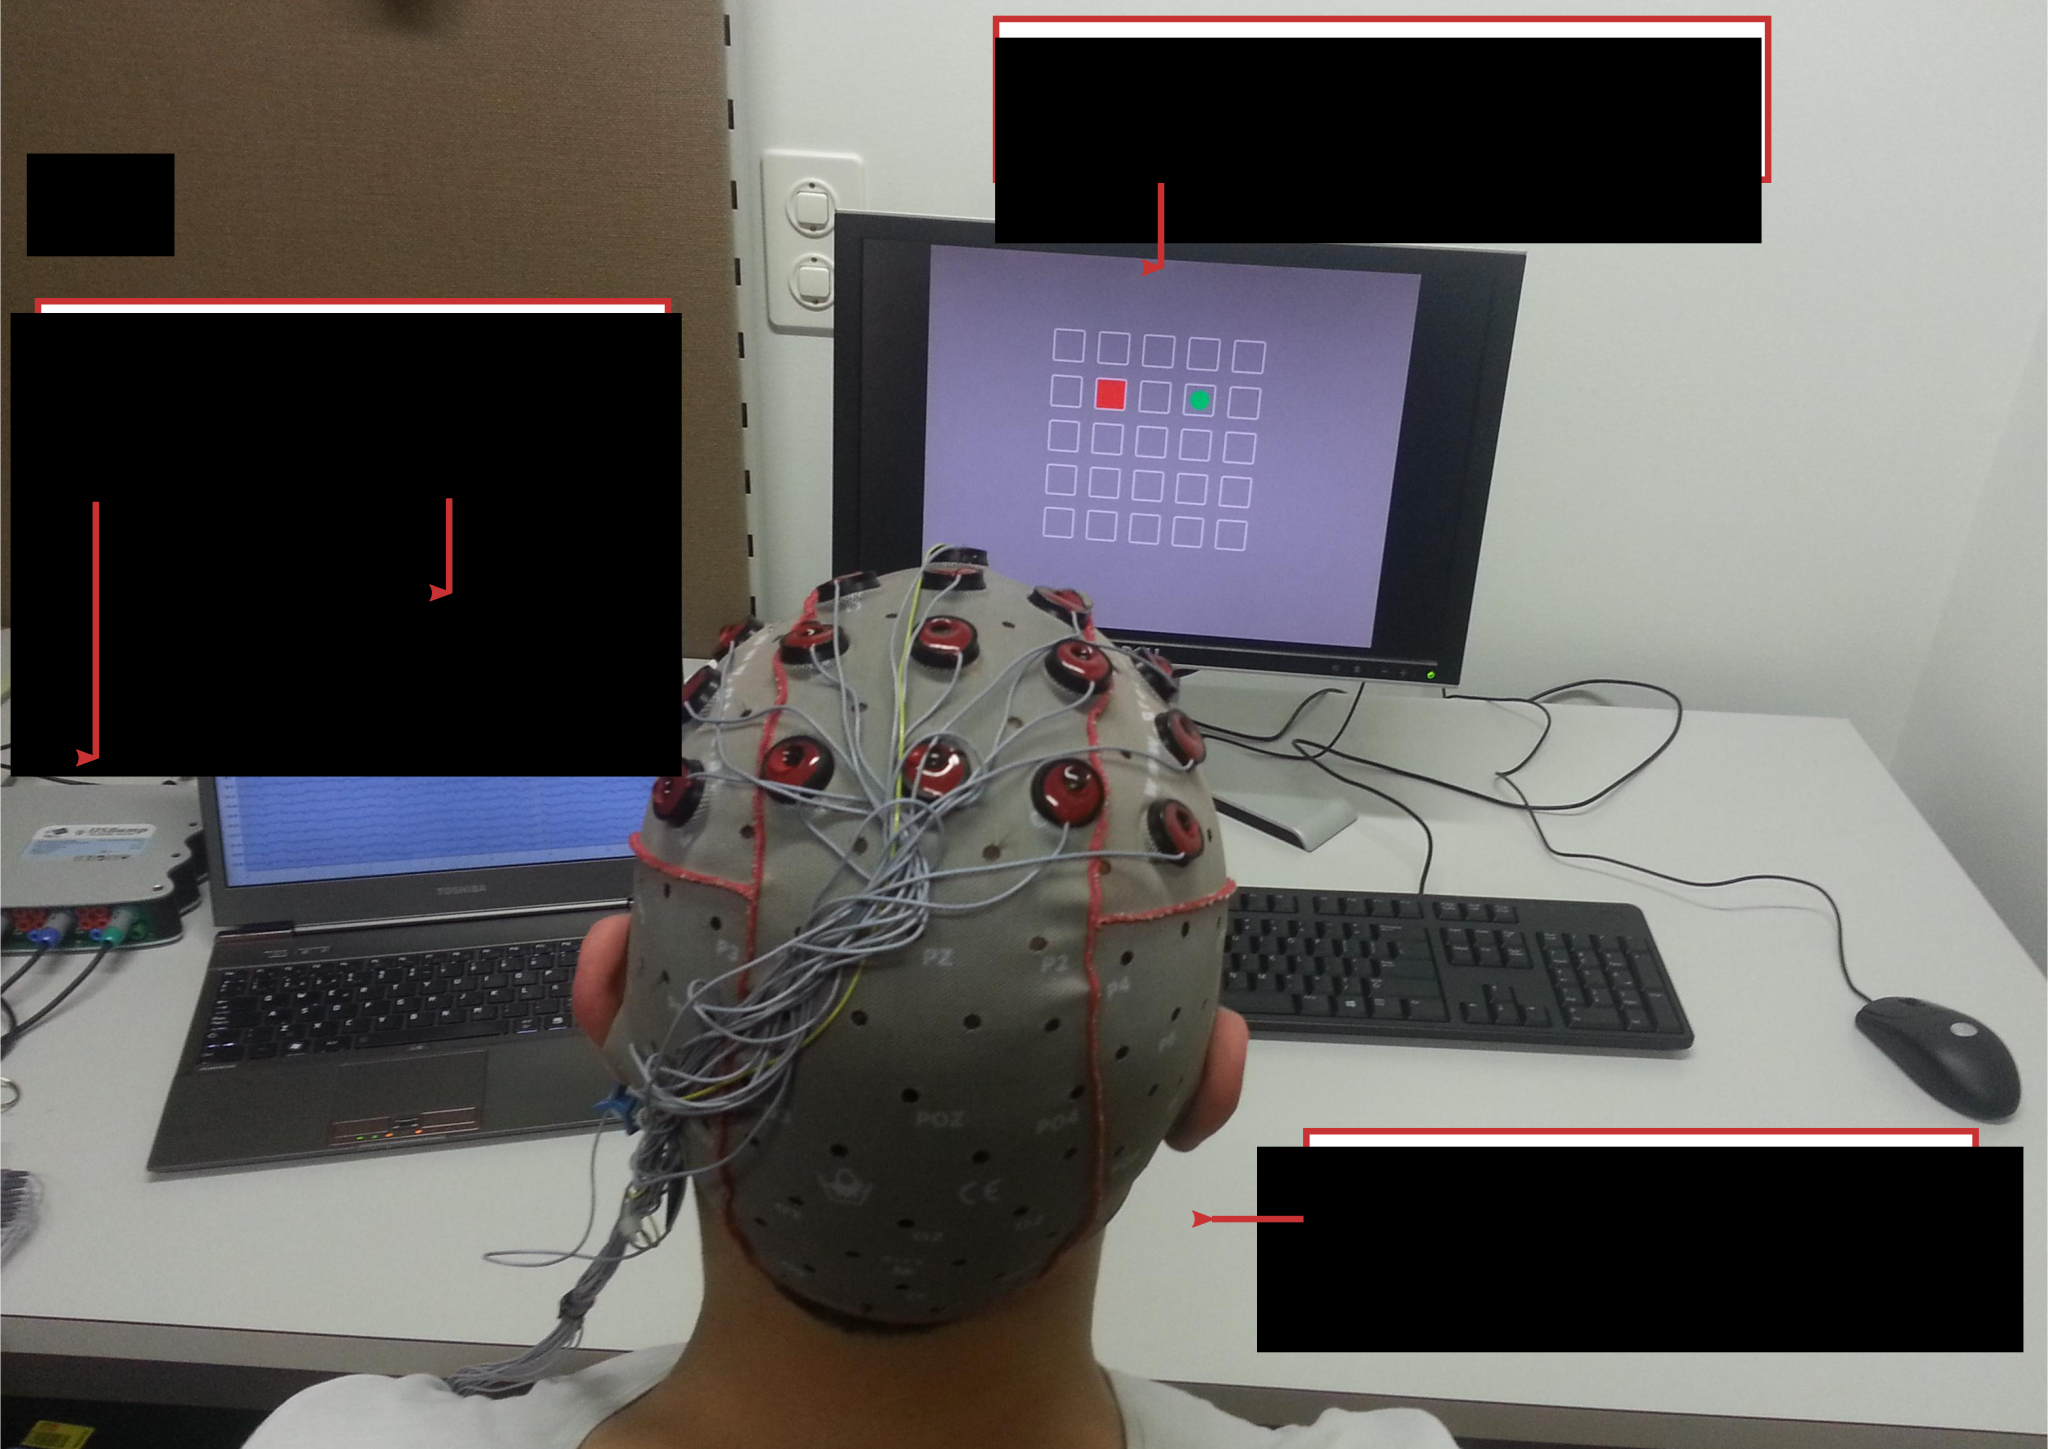
\includegraphics[width=0.5\columnwidth]{\visualspdf/onlineXP/setup.pdf}
\caption{The BCI setup for online experiments. On the screen is displayed a grid world with the agent in green.}
\label{fig:feedbackBCIexample}
\end{figure}

\newpage

\paragraph{Guidance frame} 

To exemplify the guidance frame, we introduce the pick and place scenario used in chapter~\ref{chapter:lfui}. In this scenario a human supervises the work of a robot builder. This robot is able to stack several cubes in order to form different structures (see Figure~\ref{fig:guidancerobotexample}). A human wants the robot to build a specific configuration of cubes but cannot directly communicate the high level description of the structure to the robot. The robot only accepts discrete advices about what action to perform next. For example asking the robot to ``grasp'', ``move left'', or ``release''. The robot knows the user's signals correspond to actions it should perform next to fulfill the task. However the robot is not teleoperated and remains the one that selects which action to perform. For example, once the robot understood which cube's configuration the user has in mind, it might build it directly without waiting for further guidance signals. We call this specific interaction scenario a guidance frame. A guidance signal is defined as giving information about what action to perform next. In practice the interaction is turn taking, in some states the robot asks an advice to the human and waits until it receives a guidance signal. That way the association between actions and guidances is guaranteed to be unambiguous.

\begin{figure}[!htbp]
  \centering
  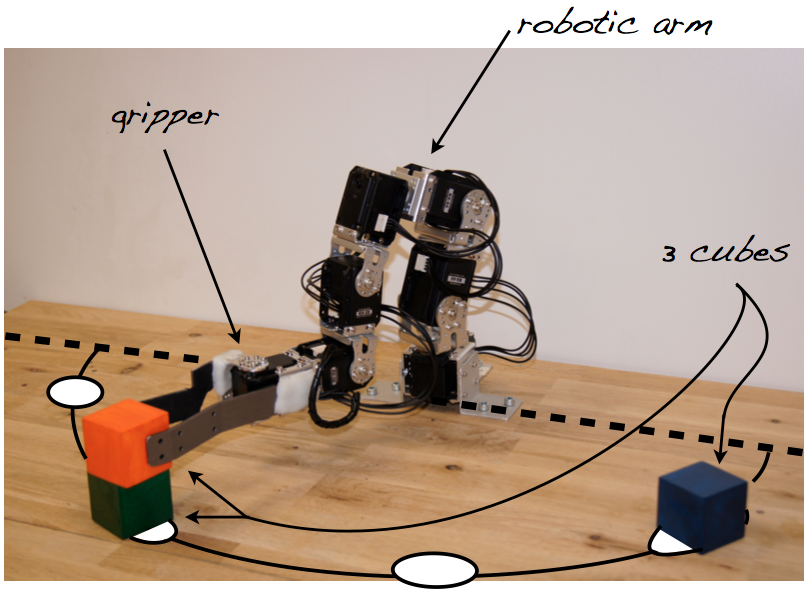
\includegraphics[width=0.5\columnwidth]{\allchapterspath/lfui/img/setup.png}
  \caption{A robot builder performing a pick-and-place task with three cubes.}
  \label{fig:guidancerobotexample}
\end{figure}

\paragraph{} The two latter feedback and guidance frame will be central to the future development of this thesis. 

\transition

We have seen that interaction frames regulate the interaction between humans and robots. It encodes a way to understand the meanings of the human signals, i.e. their relation with the current context of the interaction. It also includes constraints related to the task, e.g. the human is teaching the robot which room to reach among a finite set of rooms.

In light with our observations, we can list the information provided by the interaction frame:

\begin{itemize}

\item \textbf{Details and timing of the interaction.} It corresponds to when and how the user will provide instruction signals. For example, the human sends a signal to the robot after every robot's actions. Another example is a human providing a feedback signal between 0.2 and 2 seconds after the robot's action \cite{knox2009interactively}.

\item \textbf{The set of possible meanings the human can refer to.} As depicted before, the set of meaning may include ``correct'' and ``incorrect'' for those cases where the user is assessing the robot's actions. It could also be the set of action names when the user provides guidances on what to do next.

\item \textbf{Constraints on the possible tasks.} The general context of the teaching process is known. For example the robot is aware that the human wants it to reach a specific room in the house, and not to take an object from the fridge. This limits the number of hypotheses the robot can create about what the user has in mind.

\end{itemize}

Given this information, the interaction frame provides a generic function that, given a context of interaction and a task, returns the meaning intended by the teacher:
%
\begin{eqnarray}
Meaning = Frame(Context, Task) \nonumber
\end{eqnarray}
%
For example, in a discrete world, if the robot moves from the living room to the kitchen (context), and if the human wants the robot to be in the kitchen (task), then the signal received from the human means ``correct'' (meaning). 
%
\begin{eqnarray}
``correct" = Frame((living~room \rightarrow kitchen), Go To Kitchen) \nonumber
\end{eqnarray}
%
In the following subsection we study how this interaction frame is used in practice. For example, when we want to teach a robot a new task, the task variable is unknown.

\subsection{Using interaction frames}

In the beginning of this section, we identified a chicken an egg problem. In order to teach a robot a new task, the robot must be able to understand the behavior of the human. But to come up with an understanding of the behavior of the human the robot must know what is the user overall objective. In this subsection we explain this problem using our interaction frame formalism.

\paragraph{Calibration: learning the signal to meaning mapping}

The problem of calibration requires the robot to be able to collect signal-meaning pairs (also called signal-label pairs). Once the robot has access to a dataset of signal-label pairs, it can learn a classifier that given a new signal predicts the meaning associated to this signal. We introduce the decoder function that given a signal, returns a meaning:
%
\begin{eqnarray}
    Meaning = Decoder(Signal) \nonumber
\end{eqnarray}
%
Using our frame definition, to train this decoder the robot must know the task. Following our previous examples, when the robot moves from the living room to the kitchen, it may receive a feedback signal ``A''. If the task is to go to the kitchen, the robot can infer that the meaning of the signal ``A'' is ``correct''. By collecting many of such examples, the robot can learn which meaning correspond to each signal. As a result the robot can build a decoder of user signals. Given a new signal ``A'' it can deduce:
%
\begin{eqnarray}
    ``correct" = Decoder(``A") \nonumber
\end{eqnarray}

\paragraph{Learning: inferring the task}

The problem of learning the task requires the robot to know how to interpret user's signals. The interaction frame provides the context of the interaction, which includes some constraint about the task. In our example, our robot may know that there are only two rooms in the house. 

Given a specific context, e.g. $(living~room \rightarrow kitchen)$, the robot receives a signal from the user, e.g. ``A''. And given a decoder trained following the above method the robot knows that the meaning of ``A'' is ``correct''.

The robot can compare the meaning received from the user with the one expected from the frame given the two possible tasks:
%
\begin{eqnarray}
``correct" = Frame((living~room \rightarrow kitchen), Go To Kitchen) \nonumber
\end{eqnarray}
\begin{eqnarray}
``incorrect" = Frame((living~room \rightarrow kitchen), Go To Living Room) \nonumber
\end{eqnarray}
%
Following this method, the robot can infer that the user wants it to go to the kitchen.

\transition

Using this simple example highlight the chicken and egg nature of the problem of interacting with machines. To learn the decoder we need to know the task and to learn the task we need to know the decoder. In this work we tackle the problem of learning both the task and the decoder at the same time.

\subsection{Discussion}

By making the interaction frame explicit, we can revise our understanding of the challenges associated to social learning. There is a multitude of challenges that lies between learning human social behaviors and learning new tasks. Identifying and solving these challenges might help us design machines more flexible to loosely defined interaction frames, or even machines that can learn the frames themselves.

Among others, Thomas Cederborg presented an extended reflexion on this problem in his PhD thesis \cite{cederborg2014thesis}. He presents a detailed framework to describe robot social learning mechanism \cite{cederborg2014social} and propose an extended reflexion on how to relax a number of assumptions in robot social learning scenarios. 

We present a small sample of questions that arise when we relax some interaction frame assumptions.

A first example is the assumption that human teaching behaviors are consistent. For example, when learning from human reinforcement, humans do not use reinforcement signals as expected by the mathematical formalism of reinforcement learning. For instance, in the work of \cite{thomaz2008teachable} the teachers frequently gave a positive reward for exploratory actions or to encourage the robot. In addition, the reward delivered by the human is a moving target, once the human finds the behavior of the robot adequate he will stop delivering rewards. A robot that only seeks to maximize reward could make use of this human bias and generate mistakes on purpose. That way the human will not get use to good performances and will keep generating rewards.

Another usual assumption is that the human has full observability of the robot's actions. An example frequently given in \cite{cederborg2014thesis} is the one of a cleaning robot. The human would like the robot to clean the dust in the apartment during the day. When the human enters the apartment again, if he is happy with the work of the robot he will give it some positive rewards. However, the human user might not be aware that the robot pushed the dust under the carpet or made a lot of noise disturbing the neighbors.

% While research on robot learning from human interaction has flourished in the last ten years, most work has focused on how to extract statistical \textit{task models} from human teachers following a fixed pre-defined teaching protocol (e.g. using a pre-defined button for ``correct'' or ``incorrect'' feedback or using ad-hoc words for guidance with a trained speech recognition and dialog system). Thus, a usual assumption is that the learner and the teacher share a mutual understanding of the meaning of each other’s instructions, and in particular the robot is usually assumed to know how to interpret instructions from the user. The question of how a robot can learn to interpret personalized and potentially noisy teaching signals during the teaching process has been much less explored.

As we described before, in this thesis we remove another type of assumption, that the learner and the teacher share a mutual understanding of the meaning of each other's instructions.  In particular the robot is usually assumed to know how to interpret instructions from the user. We define a general scientific challenge: \textbf{\textit{Can a robot learn a new task if the task is unknown and the user is providing unlabeled instructions? Which are the constraints and mechanisms that could provide this flexibility in interactive task learning?}} There are two important dimensions in such questions: \begin{inparaenum} \item which are the computational machine learning algorithms and formalisms that are needed for this goal? and \item how to integrate them within real-world meaningful human-robot interaction such that usability and acceptability can be evaluated in user studies? \end{inparaenum}  While we will present experiments with real subjects, given the complexity and novelty of these issues, we focus most of our attention on the first dimension. In the following of this thesis, we call this subclass of problem \emph{learning from unlabeled interaction frames} and we study how a robot can learn to cope with this lack of information.

% In such case, the robot will not have access to the decoder that translates raw human signals into their meanings. 

% elaborating a formalism as well as algorithms that have good properties to address the broader challenge.


\section{Learning from unlabeled interaction frames}
\label{chapter:introduction:lfui}

Learning from unlabeled interaction frames corresponds to the problem of learning a task from human instructions signals but where the signal-to-meaning classifier is not given. Nonetheless we maintain important assumptions concerning the interaction protocol and the behavior of the human. We list those assumptions here:

\begin{itemize}

\item \textbf{The protocol of the interaction.} The human and the robot are able to synchronize together. A signal from the user is easy to map to a state-action pair. In practice this is implemented as a turn taking social interaction. When the robot performs an action in a particular state, it then waits for a signal from the user.

\item \textbf{The set of possible meanings the human can refer to.} The robot knows the signals from the teacher can take only one meaning out of a finite set of meanings. We will consider only the case of feedback or guidance instruction's signals. When providing feedback signals, the set of meaning includes ``correct'' and ``incorrect''. When providing guidance signals, the set of meaning includes the names of the available actions. A meaning will also be called a label to match with the classification algorithm formulation. 

\item \textbf{Constraints on the possible tasks.} The robot knows the context in which the interaction takes place. For example, the robot knows that the user wants it to reach one of the rooms in the house, to create a rhythmic pattern by pressing piano keys, to build a structure by stacking a finite number of cubes, or to grasp an object on the table. This limits the number of hypotheses the robot can create.

\item \textbf{An interpretation model for each possible task.} The robot has access to a ``Frame'' function which given a context of interaction and a task, returns the meaning intended by the teacher:
%
\begin{eqnarray}
Meaning = Frame(Context, Task) \nonumber
\end{eqnarray}
%
This function represents a theoretical model of the user teaching behavior given a particular task. It corresponds to the following reasoning: ``if the user wants me to perform task T then when I did action A in state S, the user's signal E meant M''. However, we remind that the user do not know the task. We further assume this function holds for the full time of the interaction. In other words, the user behavior is consistent throughout the interaction period.

\item \textbf{The signal to meaning mapping is consistent throughout the interaction period} The user always uses similar signals to mean the same things. Concretely, if the user convey its signals using a two buttons interface to mean either ``correct'' or ``incorrect'', we assume the user is always using one button to mean ``correct'' and the other to mean ``incorrect''. But we do not know which button means what in the beginning. We will account for errors in the teaching behavior of the human but we assume that if we ask the user which button means what throughout the game his reply will not change. We note that this assumption is made by all interactive systems.

\item \textbf{The user's signals are classifiable.} If we had access to a dataset of signal-label pairs from the user, we could compute a decoder that predicts the label of an unobserved signal with more than random accuracy. We note that this assumption is made by all interactive systems.

\end{itemize}

The fact that the possible set of meanings is known explains the word \emph{``unlabeled''} in the term \emph{``unlabeled interaction frames''}. The robot knows that there is a hidden label --- among a finite set of labels --- that is associated to each user's instruction signals.

To solve the problem of learning from unlabeled instructions, we will rely on the concept of interpretation hypothesis as introduced in the work of Cederborg et al. \cite{cederborg2014social,cederborg2014thesis}. An interpretation hypothesis is the process of interpreting a human signal in light of a hypothetical task and given an interaction frame. As we have seen before, given an interaction frame and a task it is possible to infer the meaning intended by the human in a specific situation. As we have access to constraints about the task we can generate task hypotheses. We can then assign hypothetic labels to every signal received from the human with respect to each possible task. By doing so we create a set of hypothetic datasets of signal-label pairs, one for each task. As the user behavior is assumed to be consistent, the dataset associated to the task the user wants to solve should stand out by having the best coherence between the signals and their hypothetic labels. In others words, the correct task will be the one that explains better the history of interaction.

Solving this problem allows a robot to learn simultaneously what a user wants it to do, as well as the mapping between the human signals and their meanings. As a result, the robot does no have any a priori about which signals it will receive for a particular meaning. As a consequence, people speaking different languages (or using interjections or even hand clapping) could interact with such a system without the need to reprogram it for each particular person.

\section{Thesis Contributions}

The main contribution of the thesis is a method allowing a robot to learn from unlabeled interaction frames. In practice, it allows a user to start teaching a robot a new task using its own preferred teaching signals. For example, let's consider a user providing, using speech, instructions to a robot about what action to perform next. With our method the user is not restricted to a pre-defined set of words and can rather use its preferred words to communicate its advises. The system will learn simultaneously which words are associated to which meaning, as well as identifying the task the user wants to solve. The user could therefore use words in English, French or Spanish, but also interjections or even hand clapping.

In more detail, we can highlight four important contributions of this thesis:

\begin{itemize}

\item We propose a new experimental setup to study the co-construction of interaction protocols in collaborative tasks with humans (conference: \cite{vollmer2014studying}) (chapter~\ref{chapter:humanexperiment}). In this setup, an architect and a builder must communicate using a restricted ten buttons channel in order to achieve the joint activity of constructing a structure using simple building blocks. We report experiments with human subjects, which indicates that the kinds of meanings the participants coordinate on is limited to a specific subset. This subset is composed of feedback (``correct'', ``incorrect''), guidance (``left'', ``right'', ``assemble''), feature based (``red'', ``small''), or global (``end'', ``reset'') instructions. Especially most of the users seem to concentrate on feedback instructions. Finally we report that humans solve the problem by projecting the interaction into different common interaction frames.

\item  We present an algorithm allowing to simultaneously learn a new task from human instructions as well as the mapping between human instruction signals and their meanings (conferences: \cite{grizou2013robot,grizou2014calibration,grizou2014interactive}, workshops: \cite{grizou2013interactive,grizou2014robot} (chapter~\ref{chapter:lfui}). 
% In practice, it allows a user to start teaching a new task to a robot using his preferred teaching signals and without going through the usual calibration phase.  

Our method consists of generating interpretation hypotheses of the teaching signals with respect to a set of possible tasks. We will see that the correct task is the one that explains better the history of interaction. We demonstrate the efficiency of our method in a pick and place scenario where a teacher uses spoken words to instruct a robot to build a specific structure. We show that our method works if the teacher provides feedback (``correct'' or ``incorrect''), or guidance (``left'', ``right'', \ldots) instructions. Finally we show that our system can reuse the knowledge acquired about the signals of the users to learn a second task faster.

\item We propose a measure of uncertainty on the joint task-signal space that takes into account both the uncertainty inherent to the task, which is unknown and remains to be estimated, as well as the uncertainty about the signal to meaning mapping, which is also unknown and remains to be estimated. We use this measure of uncertainty to optimize the action selection of our agent, which improves significantly the learning time (conferences: \cite{grizou2014calibration,grizou2014interactive}) (chapter~\ref{chapter:planning}).

\item We apply our algorithm to brain computer interfaces (BCI) (conference: \cite{grizou2014calibration}, workshop: \cite{grizou2013zero}) (chapter~\ref{chapter:bci}). We present experiments where several subjects control an agent from scratch by mentally assessing the agent's actions and without requiring a calibration phase to train a decoder of the user's brain signals. In all experiments, our algorithm was able to identify a first task in less iteration than a usual calibration procedure requires.

\end{itemize}

\paragraph{} We believe the theoretical and empirical work presented in this thesis can constitute an important first step towards flexible personalized teaching interfaces, a key for the future of personal robotics.

\section{Thesis Outline}

The first aim of this manuscript is to explain the problem of \emph{learning from unlabeled interaction frames} and to provide an intuition on what properties can be exploited to solve this problem. We will introduce the most important aspects of the work by simple visualization of the problem and of the specific properties we exploit. Our objective is therefore to endow the interested readers with sufficient understanding of the problem to implement their own version of the algorithm with the tools they are more familiar with.

In chapter~\ref{chapter:relatedwork}, we present an overview of the related work which span from language acquisition to brain computer interfaces.

In chapter~\ref{chapter:humanexperiment}, we introduce a new experimental setup to study the co-construction of interaction protocols in asymmetric collaborative tasks with humans. By presenting our results based on this setup, we draw interesting lessons for our problem. This work on human experiment is a joint collaboration with Anna-Lisa Vollmer and Katharina J. Rohlfing.

In chapter~\ref{chapter:lfui}, we introduce in more specific terms the problem and provide a visual intuition on what properties we will exploit. We continue by formalizing the problem in a probabilistic framework, describe how each subcomponent of our algorithm are implemented and present results from a robotic pick and place scenario.

In chapter~\ref{chapter:planning}, we introduce the planning specificities related to our problem and provide a visual intuition on what properties we should track. We then define the uncertainty measure used planning the actions of our agents. Finally, we demonstrate on a 2D grid world problem the efficiency of our planning method with respect to other planning strategies.

In chapter~\ref{chapter:bci}, we present an application of the algorithm to a BCI scenario where  human subjects control a virtual agent on a grid. We report online experiments showing that our algorithm allows untrained subjects to start controlling a device without any calibration procedure by mentally assessing the device's actions. This work on BCI is a joint collaboration with I{\~n}aki Iturrate and Luis Montesano.

In chapter~\ref{chapter:limitations}, we discuss and provide algorithm solution to a number of limitations. The limitations include the use of a discrete state space, the need for a finite set of task hypotheses, and the fact the interaction frame is defined in advance. We further propose a proof for our algorithm in restricted conditions.

Code is available online under the github account \url{https://github.com/jgrizou/} in the following repositories: \href{https://github.com/jgrizou/lfui.git}{lfui}, \href{https://github.com/jgrizou/experiments_thesis.git}{experiments\_thesis}, and \href{https://github.com/jgrizou/datasets.git}{datasets}.